%% $Id$

\documentclass[12pt]{article}

\usepackage{a4wide}
\usepackage{graphicx}
\usepackage{amsmath}

%%%%%%%%%%%%%%%%%%%%%%%%%%%%%%%%%%%%%%%%%%%%%%%%%%%%%
%% Macros for comments
\usepackage{amssymb}
\newcounter{comment}

\newcommand{\comminline}[1]{{%
\refstepcounter{comment}%
\ttfamily\small[$\blacksquare$ \textbf{\underline{Comment}
$\sharp$\thecomment:} #1]}}

\newenvironment{commblock}%
{\refstepcounter{comment}%
\begin{quote}\renewcommand{\baselinestretch}{1}
\ttfamily\small$\blacksquare$ \textbf{\underline{Comment} $\sharp$\thecomment:}}%
{\end{quote}}


\newcommand{\replline}[1]{{
%\refstepcounter{comment}%
\ttfamily\small[$\blacktriangleright$ \textbf{\underline{Reply}
$\sharp$\thecomment:} #1]}}

\newenvironment{replblock}%
{%\refstepcounter{comment}
\begin{quote}\renewcommand{\baselinestretch}{1}
\ttfamily\small$\blacktriangleright$ \textbf{\underline{Reply} $\sharp$\thecomment:}}%
{\end{quote}}
%%%%%%%%%%%%%%%%%%%%%%%%%%%%%%%%%%%%%%%%%%%%%%%%%%%%%

\begin{document}

\title{\texttt{gepard} --- Compton form factors and observables
                            by evolving moments of GEneral PARton Distributions}
\author{Version: 0.9}
\date{\today}
\maketitle

\begin{abstract}
Fortran package \texttt{gepard} calculates singlet Compton form factor
$\mathcal{H}$ and corresponding Compton cross-sections, as well as
DIS form factor $F_2$ by evolving GPDs in conformal moment space from an ansatz shape
specified at some input scale.  Together
with \texttt{Minuit} minimization subroutine GPD parameters can be fitted to
experimental DVCS and DIS data. For installation instructions and
basic usage, see README file coming with the package.
\end{abstract}

\tableofcontents
\clearpage

\section{Mellin-Barnes representation of relevant observables}

\subsection{DVCS formulas}  

For small $\xi$, DVCS cross section can be approximated by 
\begin{equation}
\frac{d \sigma_{\rm T}}{d t} = \frac{4 \pi \alpha^2 W^2}{(W^2 + \mathcal{Q}^2)
(2 W^2 + \mathcal{Q}^2)^2} | ^{\rm S}\mathcal{H}(\xi, t, \mathcal{Q}^2)|^2 \Bigg|_{\xi
= \frac{\mathcal{Q}^2}{2 W^2 + \mathcal{Q}^2}} \;,
\label{eq:parsigma}
\end{equation}
where singlet Compton form factor $^{\rm S}\mathcal{H}$ in Mellin-Barnes representation is given by
\begin{equation}
{^{\rm S}{\cal H}}(\xi,\Delta^2,{\cal Q}^2)
= \frac{1}{2i}\int_{c-i \infty}^{c+ i \infty}\!
dj\,\xi^{-j-1} \left[i + \tan \left(\frac{\pi j}{2}\right) \right]
\mbox{\boldmath $C$}_{j}({\cal Q}^2/\mu^2,\alpha_s(\mu)) 
\mbox{\boldmath $H$}_{j} (\xi,\Delta^2,\mu^2) \;.
\label{eq:CFF}
\end{equation}
DVCS Wilson coefficients $\mbox{\boldmath $C$}_{j}({\cal Q}^2/\mu^2,\alpha_s(\mu))$
are given in Eq. (18) of \cite{Kumericki:2006xx}, while moments of
GPD $\mbox{\boldmath $H$}_{j} (\xi,\Delta^2,\mu^2)$ should be specified
by the user in subroutine \texttt{HJ}, as described in subsection \ref{ssect:ansatz}.

In practice it is good to use Mellin-Barnes contour of the form displayed
on Fig.~\ref{fig:MellinBarnes}, with point on the contour given
by $j=c+ye^{i\phi}$, with real parameters $c$ and $\phi$.
The usual textbook Mellin-Barnes contour is obtained by
using $\phi = \pi/2$, but, say, $\phi = 3\pi /4$ gives faster
convergence. As long as no poles are crossed value of the
integral should not depend on the value of $c$. One can
try different values of $c$ and $\phi$ to get best numerical
properties. 
By default, in \texttt{init.f} it is set $c$ = 0.5 and $\phi = 3\pi/4$.

\begin{figure}[ht]
\begin{center}
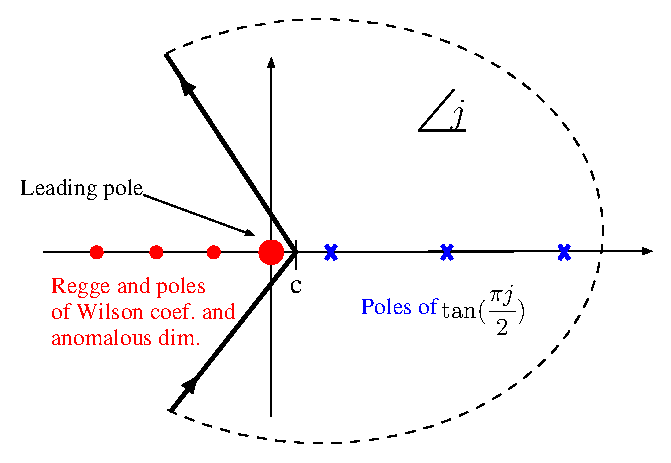
\includegraphics[scale=1.0]{MellinBarnes}
\end{center}
\caption{Contour of the Mellin-Barnes integration.}
\label{fig:MellinBarnes}
\end{figure}


To write the Mellin-Barnes integral in (\ref{eq:CFF}) as an integral
over real variable $y$, one can employ Schwartz reflection principle to
actually integrate over only one of two legs on Fig.~\ref{fig:MellinBarnes}
and write
\begin{multline}
{^{\rm S}{\cal H}}(\xi,\Delta^2,{\cal Q}^2) =
\Im\! m\:  e^{i\phi} 
\int_{0}^{\infty} dy \, \xi^{-j-1}
\tan\big(\frac{\pi j}{2}\big)
\mbox{\boldmath $C$}_{j}({\cal Q}^2/\mu^2,\alpha_s(\mu)) 
\mbox{\boldmath $H$}_{j} (\xi,\Delta^2,\mu^2) \\
+ i\: \Im\! m\:  e^{i\phi} 
\int_{0}^{\infty} dy \, \xi^{-j-1}
\mbox{\boldmath $C$}_{j}({\cal Q}^2/\mu^2,\alpha_s(\mu)) 
\mbox{\boldmath $H$}_{j} (\xi,\Delta^2,\mu^2) 
\Bigg|_{j = c + y e^{i\phi}}
\label{<Hformula>}
\end{multline}

\subsection{DIS formulas}  

Similarly, deeply inelastic scattering singlet form-factor ${^{\rm S}\!{F_2}}$ is given by
\begin{eqnarray}
{^{\rm S}\!{F_2}}(\xi,{\cal Q}^2)
&\!\!\!=\!\!\!& \frac{Q_{S}^2}{2 \pi i}\int_{c-i \infty}^{c+ i \infty}\!
dj\,\xi^{-j}
\mbox{\boldmath $C$}^{\rm DIS}_{2,j}(Q^2/\mu^2,\alpha_s(\mu))
\mbox{\boldmath $H$}_{j} (\xi=0,\Delta^2=0,\mu^2) \nonumber \\[2ex]
&\!\!\!=\!\!\!& \frac{Q_{S}^2}{\pi}\, \Im\! m\: e^{i\phi}
\int_{0}^{\infty} dy\:  \xi^{-j}
\mbox{\boldmath $C$}^{\rm DIS}_{2,j}(Q^2/\mu^2,\alpha_s(\mu))
\mbox{\boldmath $H$}_{j} (\xi=0,\Delta^2=0,\mu^2) 
\Bigg|_{j = c + y e^{i\phi}}
\label{<F2formula>}
\end{eqnarray}
DIS Wilson coefficients $\mbox{\boldmath $C$}^{\rm DIS}_{2,j}(Q^2/\mu^2,\alpha_s(\mu))$
are given e.g. in \cite{vanNeerven:2000uj}.

\subsection{Numerical Mellin-Barnes Integration}  
\label{ssect:Integration}
Numerical integration is performed in a way very similar to the one described in
\cite{Vogt:2004ns}: Integrand is largest and
fluctuates most rapidly around zero, mostly due to the factor $\xi^{-j}$. As we
move away from real axis, both
amplitude and oscillation frequency decrease exponentially.
This leads us to divide integration region in exponentially expanding intervals
defined by points:
\begin{align*}
0 \,\ldots\, 0.01 \,\ldots\, 0.025\,\ldots\, 0.067\,\ldots\,& 0.18\,\ldots\, 0.5\,\ldots\, 1.3\,\ldots\, 3.7\,\ldots\, 10&
\qquad \text{(for \texttt{SPEED=1})} \\
0  \,\ldots\, 0.025\,\ldots\,& 0.18\,\ldots\, 1.3 \,\ldots\, 10&
\qquad \text{(for \texttt{SPEED=2})} \\
0  \,\ldots\,& 0.18 \,\ldots\, 3.7&
\qquad \text{(for \texttt{SPEED=4})} \\
\label{<intervals>}
\end{align*}
Here \texttt{SPEED} is one of \texttt{gepard}'s initialization parameters which
controls speed and accuracy of evaluations, see Section \ref{ssect:GEPARD.INI}.
On each segment, standard 8-point Gaussian integration is employed, according
to Eq. (25.4.30) from \cite{AbS65}.
Thus for \texttt{SPEED}=1,2, and 4 we use in total 64, 32, and 16
integration points, respectively. 

During the initialization phase, coordinates of points on Mellin-Barnes contour and 
their Gaussian-integration weights
are put on the Fortran common blocks, together with corresponding values of
the moments of Wilson coefficients and anomalous dimensions. Thus these
time-demanding evaluations are performed only once.

\begin{commblock}
It would be good to calculate also evolution operator during the initialization phase.
This would be reasonably easy to implement for fits with fixed $\mathcal{Q}_{0}^2$, 
where evolution is needed only for small number of fixed ratios 
$\alpha_{s}(\mathcal{Q})/\alpha_{s}(\mathcal{Q}_0)$. (In the general case, one could
maybe make interpolation function for evolution operator.)
Looking at the execution profile of the present code, i.e. how much time is spent
in particular subroutines, it seems to me that by such improvements one can hope
for a speed-up of about factor 5-8. This could be the next step if the present
speed turns out to be insufficient.
\end{commblock}


\subsection{Ansatz for GPD $\mbox{\boldmath $H$}_{j} (\xi,\Delta^2,\mathcal{Q}_{0}^2)$}
\label{ssect:ansatz}

User has to provide values of moments of GPDs $\mbox{\boldmath $H$}_{j} 
(\xi,\Delta^2,\mathcal{Q}_{0}^2)$
on an input scale by defining subroutine \texttt{HJ} which has the synopsis
\begin{verbatim}
      SUBROUTINE HJ(J, FCM)

      DOUBLE COMPLEX J, FCM(2)
      DOUBLE PRECISION XI, DEL2, Q2, Q02
      COMMON / KINEMATICS /  XI, DEL2, Q2, Q02
\end{verbatim}
Input to the subroutine is the complex conformal moment \texttt{J} (i.e. coordinates of a point
on the Melin-Barnes contour), and kinematical parameters $\xi$, $t=\Delta^2$, $\mathcal{Q}^2$
(not used), and $\mathcal{Q}_{0}^2$ (these last four via common block), while output should 
be corresponding values
\begin{align}
\texttt{FCM(1)}& =\, ^{\Sigma}\!H_{j} (\xi,\Delta^2,\mathcal{Q}_{0}^2)  \\
\texttt{FCM(2)}& =\, ^{G}\!H_{j}(\xi,\Delta^2,\mathcal{Q}_{0}^2) \,.
\label{eq:FCM}
\end{align}
In the subroutine \texttt{HJ} provided by default, there is already implemented ansatz
\begin{equation}
^{a}\!H_{j}(\xi,\Delta^2,\mathcal{Q}_{0}^2) = 
N_a F_{a} (\Delta^2) \frac{ {\rm B}\big(1+j-\alpha_{a}(\Delta^2), \mathcal{P}_a\big)}{
{\rm B}\big(2-\alpha_{a}(0),\mathcal{P}_a\big)}\;, \qquad a = \Sigma, G \,
\label{eq:ansatzFIT}
\end{equation}
where $\mathcal{P}_\Sigma$ = 8,  $\mathcal{P}_G$ = 6, $\alpha_{a}(\Delta^2) =
\alpha_{a}(0) + 0.25 \Delta^2$  and 
\begin{equation}
F_{a} (\Delta^2) = \left(1 - \frac{\Delta^2}{m_{a}^2}\right)^{-3} \,.
\label{eq:F}
\end{equation}
Six free parameters of this ansatz ($N_a$, $m_a$ and $\alpha_{a}(0)$, for  $a = \Sigma, G$),
can either be fixed, or provided by the minimization routine for fitting, see
Fig.~\ref{fig:MINUIT.CMD}.


\section{\texttt{gepard} ingredients}

\begin{itemize}
\item Collection of QCD anomalous dimensions and Wilson coefficients for
unpolarized DIS up to NNLO which can be used for calculating DVCS form factors
in $\overline{CS}$ scheme. For detailed description of (Mathematica) version of
corresponding functions and sources, see the document \texttt{adacf.pdf}.
Collection of QCD anomalous dimensions and Wilson coefficients for singlet DVCS form factors
in $\overline{MS}$ up to NLO.

\item
The evolution of GPDs up to NLO in $\overline{CS}$ scheme. $\overline{MS}$
evolution to be included.

\item 
Mellin-Barnes representation for DVCS form-factors.
\end{itemize}

For calculating and testing DVCS form factors and observables the programs \texttt{test},
\texttt{auxtest}, \texttt{radcorr}, and \texttt{scaledep} are provided at the
moment.

For fitting the GPD parameters using Minuit, as well as for calculating observables (by
fixing all parameters to desired value), the program \texttt{fit} is provided.

\section{Initialization files}
\label{sec:init}

Execution of \texttt{gepard} routines depends on the initialization parameters specified in
the following files
\begin{itemize}
\item  \texttt{GEPARD.INI} --- main initialization for all routines
\item  \texttt{FIT.INI} --- which sets of data are used in fits
\item \texttt{MINUIT.CMD} --- Minuit minimization batch file
\item \emph{data files} --- as specified in \texttt{FIT.INI}
\end{itemize}
The format and contents of these files should be mostly clear by looking at provided
examples, and detailed explanations follow in the next subsections.

\textbf{NB:} Note that various constants in these files should be specified
according to Fortran 77 standard! Thus, integers should be without dot (e.g.
\texttt{1}), double precision values with dot and \texttt{'D'} (e.g.
\texttt{1.D0}), while character constants (i.e. strings) should be enclosed in
single quotation marks.

\subsection{\texttt{GEPARD.INI}}
\label{ssect:GEPARD.INI}

File has the structure displayed on Fig.~\ref{fig:GEPARD.INI}.
Only the first column is read by the program and it contains
values of internal Fortran variables specified in the second column and
shortly described in the third one. 
Columns two and three are just convenient reminders for the user. 

\begin{figure}[t]
\begin{center}
\hrule
\begin{verbatim}

    2          SPEED        1(most accurate), 2 or 4(fastest)
    1          P            N^{P}LO order (0, 1 or 2)
    3          NF           number of active flavours
    0.05D0     AS0          value of astrong/(2 Pi) at 2.5 GeV^2
    1.D0       RF2          ratio {\cal Q}^2/{\mu_{f}^2}
    1.D0       RR2          ratio {\cal Q}^2/{\mu_{r}^2}
    'CSBAR'    SCHEME       
    'FIT'      ANSATZ       GPD ansatz (see parwav.f subroutine HJ)

\end{verbatim}
\hrule
\end{center}
\caption{Example of initialization file \texttt{GEPARD.INI}}
\label{fig:GEPARD.INI}
\end{figure}


\begin{itemize}
\item
\texttt{SPEED} --- \emph{Integer}. Controls the speed and accuracy of the execution. Values can
presently be only 1, 2, and 4, where 1 is the most accurate and at the
same time the slowest case.
As described in Section \ref{ssect:Integration}, \texttt{SPEED} controls the number
of segments in which Mellin-Barnes integration contour is divided before 8-point
Gaussian integration is performed on each segment. It also controls number of
points used for Gaussian integration of partial Compton cross-section. This
number is 8/\texttt{SPEED}.  Thus, the total speed of fitting is approximately
proportional to the
value of \texttt{SPEED}. 

The choice \texttt{SPEED} = 1 guarantees cca. four
correct significant digits for observables for $10^{-6} \le \xi \le 10^{-1}$,
\texttt{SPEED} = 2 gives cca. two correct digits, while \texttt{SPEED} = 4
can produce inaccuracies of up to 40-50 \%, but can also give 2-3 correct
digits, depending on what is calculated.
\comminline{This is just a first assessment based on few tries. One should at
some point make extensive analysis of accuracy of routines.}.

\item
\texttt{P} --- \emph{Integer}. Perturbation theory approximation level. 0 = LO, 1 = NLO, and
  2 = NNLO. Because most of the costly evaluations are performed just once,
  during the initialization phase, NLO and NNLO fits take approximately the
  same time, while LO is cca. four times faster. \comminline{This is based
  on just one test, with \texttt{SPEED} = 2.}

\item
\texttt{NF} --- \emph{Integer}. Number of active quark flavors

\item
\texttt{AS0} --- \emph{Double precision}. Value of $\alpha_{\rm s}(2.5
\textrm{GeV}^2)/(2 \pi)$. For various test, as well as in
\cite{Kumericki:2006xx} value 0.05 vas used. More realistic value is 0.0536,
which corresponds to $\alpha(M_Z) = 0.117$. \comminline{Check this value!} 

\item
\texttt{RF2} --- \emph{Double precision}. $ {\cal Q}^2/{\mu_{f}^2}$ i.e. ratio
of photon virtuality and factorization scales squared

\item
\texttt{RR2} --- \emph{Double precision}. $ {\cal Q}^2/{\mu_{r}^2}$ i.e. ratio
of photon virtuality and renormalization scales squared

\item
\texttt{SCHEME} --- \emph{Character*5}. Renormalization scheme label. Can presently be \texttt{'CSBAR'} or
\texttt{'MSBAR'} corresponding to $\overline{CS}$ and $\overline{MS}$ schemes, respectively,
but note that evolution is at the moment implemented only for \texttt{'CSBAR'} scheme.

\item
\texttt{ANSATZ} --- \emph{Character*6}. Label of ansatz for conformal moments of GPDs on input scale. 
It should correspond to one  \texttt{IF\ldots ELSE IF} stanza in subroutine
\texttt{HJ} in file \texttt{parwav.f}. Defaultly implemented ansaetze are
\texttt{TOY} (used in some old development Mathematica notebooks), \texttt{SOFT} and \texttt{HARD},
corresponding to ansaetze from \cite{Kumericki:2006xx}, and \texttt{FIT}, corresponding
to ansatz used for fitting, see description of \texttt{MINUIT.CMD} below.

\end{itemize}

Note that \texttt{GEPARD.INI} is meant to be read at the very beginning of the
program execution, and values specified inside can be overridden later. For
example, provided program \texttt{radcorr}, which calculates ratio of NNLO to NLO
radiative corrections, ignores values of \texttt{P}, \texttt{SCHEME} and
\texttt{ANSATZ} in \texttt{GEPARD.INI}, and sets them itself.


\subsection{\texttt{FIT.INI}}

\begin{figure}[t]
\begin{center}
\hrule
\begin{verbatim}

      'testfit'
      '/VCPS'  2  3
      'START'
      'DVCS1.DAT'
      'DVCS2.DAT'
      'DVCS3.DAT'
      'DVCS4.DAT'
      'DVCS5.DAT'
      'DVCS6.DAT'
      'STOP'
      'DIS1.DAT'
      'DIS2.DAT'
      'DIS3.DAT'
      'DIS4.DAT'

\end{verbatim}
\hrule
\end{center}
\caption{Example of initialization file \texttt{FIT.INI}}
\label{fig:FIT.INI}
\end{figure}

File has the structure displayed on Fig.~\ref{fig:FIT.INI}.


\begin{itemize}

\item
1$^{\rm st}$ line (\texttt{OUTFILE}) --- \emph{Character*20}. Name of the file(s) used for output.
There are usually three output files:
\begin{itemize}
\item \texttt{OUTFILE.min}  ---  Output of Minuit routines (When run in batch mode. When
run in the interactive mode one can somehow log the terminal output. For example,
on Linux, by issuing command \texttt{script filename} before the run, and
\texttt{exit})
\item \texttt{OUTFILE.out}   ---  Final fit results in tabular form, as shown on
Fig.~\ref{fig:fitout}
\item \texttt{OUTFILE.ps}    ---  Same information as in \texttt{OUTFILE}.out but 
in graphical form, as shown on
Fig.~\ref{fig:fitps}  (This works only if you have PGPLOT library. If not, use
executable \texttt{fit\_nopgplot}.)
\end{itemize}

\item 
2$^{\rm nd}$ line (\texttt{OUTFORMAT, XPANELS, YPANELS}) ---  \emph{Character*20, Integer, Integer}.
\texttt{OUTFORMAT} specifies which graphical driver should be used according to PGPLOT conventions. Possible
values depend on your installation of PGPLOT. Some useful values are
  \begin{itemize}
  \item \texttt{'/CPS'}  will get output into landscape color Postscript file 
  \item \texttt{'/VCPS'}  will get output into portrait color Postscript file 
  \item \texttt{'/XSERVE'} will get output in an X window (may not work on MS Windows, and
   on Linux there could be problems when there are more than one page of graphs)
  \end{itemize}
On one physical page graphs will be arranged on a grid \texttt{XPANELS} 
$\times$ \texttt{YPANELS}.
If PGPLOT is not used, this line is ignored but have to be present and formatted correctly.

\item
Other lines (\texttt{DATAFNAME}) --- \emph{Character*20}. Names of
files containing the experimental data to be fitted to (see next
section for the format of these data files), or strings \texttt{'START'} and \texttt{'STOP'}. 
Only files between \texttt{'START'}
and \texttt{'STOP'} rows will be included in actual fits, while everything beyond
\texttt{'STOP'} is ignored, see example on Fig.~\ref{fig:FIT.INI}.
This facilitates easy selection of data for different fits.
\end{itemize}


\subsection{\texttt{MINUIT.CMD}}

\begin{figure}[t]
\begin{center}
\hrule
\begin{verbatim}

        0   <--  1=INTERACTIVE   0=BATCH 
        SET TITLE
           Fitting to H1/ZEUS DVCS and DIS data
        PARAMETERS
        1  'NG        '   0.3d0     .1d0
        2  'NSEA      '   0.2d0     .1d0
        3  'MG        '   1.0d0     .1d0 
        4  'MSEA      '   1.0d0     .1d0
        5  'ALPHA0G   '   1.0d0     .1d0
        6  'ALPHA0SEA '   1.0d0     .1d0
        7  'Q20       '   1.0d0     .1d0

        fixed 3 4 7
        migrad
        cali 3

\end{verbatim}
\hrule
\end{center}
\caption{Example of Minuit batch file \texttt{MINUIT.CMD}}
\label{fig:MINUIT.CMD}
\end{figure}

\texttt{MINUIT.CMD} is a file containing Minuit batch commands. Its format is explained in
Minuit manual \cite{Minuit}, Section 3.2.1. The only difference with respect to the
standard Minuit batch file is that first line has to contain integer 1 or 0 as a first
item. This controls whether one will do an interactive Minuit session, or not.
\comminline{At the beginning of the interactive part, one must issue two user-unfriendly
command, as instructed by the program. This will be made more elegant one day.}
Interactive Minuit session can be very powerful, after one carefully reads Minuit manual.

Second and third line are just giving some label to Minuit session.

Then comes the part where fit parameters are specified.
If one uses default \texttt{ANSATZ = 'FIT'} in
\texttt{GEPARD.INI}, then this part should look like on
Fig.~\ref{fig:MINUIT.CMD}. One could than only change initial values of parameters
(column 3), and maybe their starting step size (column 4). This \texttt{ANSATZ = 'FIT'} 
corresponds to ansatz described in Section \ref{ssect:ansatz}.  

Last part of this file contains Minuit command instructions. E. g. in the
example on Fig.~\ref{fig:MINUIT.CMD} one first fixes parameters number 3, 4,
and 7 (i.e. \texttt{MG}, \texttt{MSEA} and \texttt{Q20} are held at 1.0),
than performs minimization using \texttt{migrad} algorithm,
and finally prints (to the file \texttt{FIT.OUT}), and maybe plots (to the file specified in
\texttt{FIT.INI}) the results of the fit.

\subsection{Data files}

\begin{figure}[t]
\begin{center}
\hrule
\begin{verbatim}

        'SIGMA'                    YOBS
        89.d0                      W
        -1.                        Q2
        6                          N
        7.5   5.42  0.33  0.32 
        12.5  2.64  0.22  0.12 
        20    1.23  0.14  0.06 
        32.5  0.59  0.12  0.04 
        55    0.2   0.08  0.025 
        85    0.16  0.09  0.03


        *     DVCS4  [ZEUS, Phys.Lett.B573:46-62,2003, hep-ex/0305028]
        *       X = Q2,   Y = SIG   (TCUT = - \inf GeV ???)
        *       W = 89 GeV

\end{verbatim}
\hrule
\end{center}
\caption{Example of an experimental data file \texttt{DVCS4.DAT}.}
\label{fig:DVCS4.DAT}
\end{figure}

Names of these files should be specified in \texttt{FIT.INI}.
Each data file has the structure displayed on Fig.~\ref{fig:DVCS4.DAT}. In the first
four rows only the first item is read by the program and the second one
(corresponding to internal Fortran variable) is just convenient user
documentation.

\begin{itemize}
\item 
1$^{\rm st}$ row (\texttt{YOBS}) --- \emph{Character*8}. Label of the observable
corresponding to the ``y--axis'' of data. Implemented are labels
  \begin{itemize}
  \item \texttt{'PARSIGMA'} --- Partial Compton cross section $d\sigma/d t$  
  \item \texttt{'SIGMA'} --- Total Compton cross section $\sigma$  
  \item \texttt{'F2'} --- Deeply inelastic scattering form-factor $F_2$  
  \end{itemize} 
(By the way, only first two characters of label strings are significant.)


\item 
2$^{\rm nd}$ row (\texttt{W} or \texttt{X\_BJ}) --- \emph{Double precision}.
In the case of Compton scattering (i.e. \texttt{YOBS} = \texttt{'PARSIGMA'} or
\texttt{YOBS} = \texttt{'SIGMA'}) here is $\gamma^*$ -- proton invariant mass
$W$ (not squared!). In the DIS case (i.e. \texttt{YOBS} = \texttt{'F2'})
here is Bjorken $x$.

\item 
3$^{\rm rd}$ row (\texttt{Q2}) --- \emph{Double precision}. $\mathcal{Q}^2$
for Compton scattering or $Q^2$ for DIS.

Note the following important convention: If one of the quantities that should
be specified in rows 2 or 3 is actually ``x--axis'' of data, this fact
should be specified by putting the \emph{negative number} in the corresponding row!
In other words:
\begin{itemize}
\item 
For \texttt{YOBS} = \texttt{PARSIGMA}, ``x--axis'' variable is 
always $-t = - \Delta^2$, so there are no negative values.
\item 
For \texttt{YOBS} = \texttt{SIGMA}, ``x--axis'' variable is 
either $W$ or $\mathcal{Q}^2$ and corresponding row should have negative number.
\item 
For \texttt{YOBS} = \texttt{F2}, ``x--axis'' variable is 
either Bjorken $x$ or $Q^2$ and corresponding row should have negative number.
\end{itemize}
Thus, the example data on Fig.~\ref{fig:DVCS4.DAT} corresponds to
measurements of total Compton cross section $\sigma(W, \mathcal{Q}^2)$, with
fixed $W = 89\, \textrm{GeV}$, and variable $\mathcal{Q}^2$.

\item 
4$^{\rm th}$ row (\texttt{N}) --- \emph{Integer}. Number of measurements that
follow. Only \texttt{N} next lines will be taken into account, and the
rest of the file is ignored and can be used for comments.

\item
Measurement rows. They consist of four floating point numbers each,
standing for 
\[
 x \qquad y(x) \qquad \Delta y_{\rm stat} \qquad
\Delta y_{\rm syst} \;.
\]
Statistical and systematical errors are combined in quadrature for fitting.

\end{itemize}


\section{An example run}

In the directory where all initialization files named in Section~\ref{sec:init} are
placed one runs executable \texttt{fit}. When minimization is over, and results
printed out (e.g. by Minuit commands \texttt{stop, return, cali 3, \dots}), one gets
files: \texttt{OUTFILE.min} (if in batch mode),
\texttt{OUTFILE.out}, and \texttt{OUTFILE.ps} (if PGPLOT is used), where \texttt{OUTFILE}
is specified in the first line of \texttt{FIT.INI}.
The file \texttt{OUTFILE.min} contains the standard output of Minuit routines.
The file \texttt{OUTFILE.out} contains the numbers from each data file, together with
resulting fit value \texttt{Y(X)\_FIT},
and last column says how many sigmas is fit value different from experiment.
One stanza from such file is displayed on Fig.~\ref{fig:fitout}.

\begin{figure}[ht]
\begin{center}
\hrule
\small
\begin{verbatim}

 ------------------------------------------------------------------------
                                    DIS3.DAT                         
      X           Y(X)_FIT      Y(X)_EXP   DY_EXP    (FIT-EXP)/DY_EXP 
 ------------------------------------------------------------------------ 
   0.000200        1.2578        1.2150      0.08         0.5
   0.000320        1.1293        1.0890      0.06         0.7
   0.000500        1.0178        1.0330      0.07        -0.2
   0.000800        0.9110        0.9230      0.05        -0.2
   0.001300        0.8118        0.8110      0.06         0.0
   0.002000        0.7330        0.7700      0.06        -0.6
   0.003200        0.6567        0.5620      0.05         1.8
   0.005000        0.5934        0.6480      0.06        -0.9
   0.008000        0.5359        0.5640      0.06        -0.5 

\end{verbatim}
\hrule
\end{center}
\caption{Example of a part of resulting fit file \texttt{example.out}}
\label{fig:fitout}
\end{figure}

If one has PGPLOT library compiled in, than this fits are also graphed,
in the file \texttt{OUTFILE.ps}. Example graph is shown on Fig.~\ref{fig:fitps}.

\begin{figure}[t]
\begin{center}
\includegraphics[scale=0.52]{examplefit}
\end{center}
\caption{Example of a fit to DIS data.}
\label{fig:fitps}
\end{figure}


\section{Advanced usage and modifications}

\begin{itemize}
\item If one wants to introduce the relations between fitting parameters, they
can be entered in Fortran programs \texttt{dvcs.f} and \texttt{f2.f}.
The number of parameters will decrease and some fitting parameters 
will be ``dummies'' (their value will not be used at all). 
Although they are irrelevant now, they should be made as
``fixed'' in \texttt{MINUIT.CMD}
\end{itemize}


\section{Algorithmic structure of \texttt{gepard} and its subroutines}

Calling graph of subroutines for executable \texttt{fit} is displayed on
Fig.~\ref{fig:callgraph}. Each subroutine,
function and main program is described in the extended \texttt{gepard-api.pdf} documentation,
as well as hyperlinked HTML documentation produced by \texttt{robodoc} automatic
documentation generator.

\begin{figure}[ht]
\begin{center}
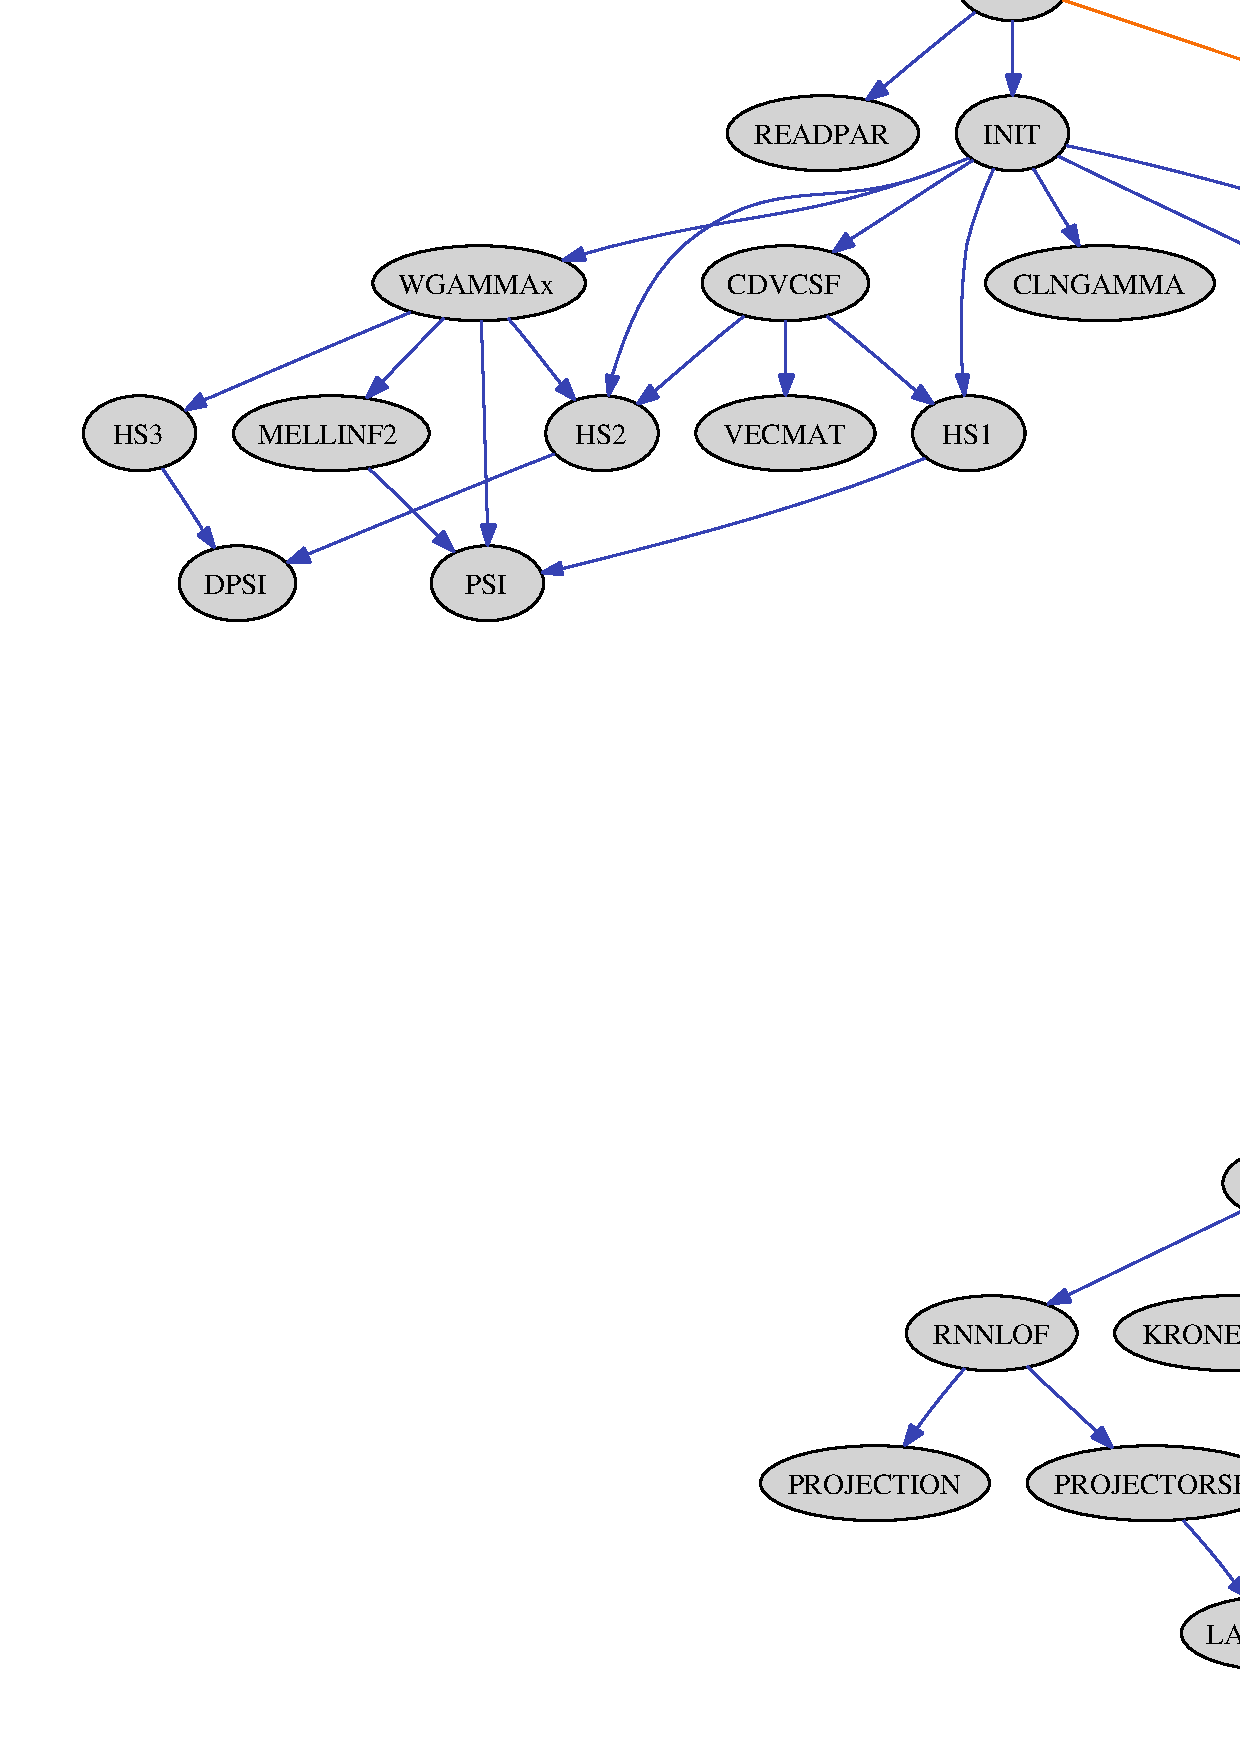
\includegraphics[scale=0.52]{callgraph}
\end{center}
\caption{Calling graph}
\label{fig:callgraph}
\end{figure}




%\bibliographystyle{h-physrev4}
\bibliographystyle{$HOME/tex/inputs/JHEP-2}
%\bibliographystyle{mynatbib}
\bibliography{$HOME/Lit/kkumer}



\end{document}

